%%%%%%%%%%%%%%%%%%%%%%%%%%%%%%%%%%%%%%%%%%%%%%%%%%%%%%%%%%%%%%%%%%%%%%%%%%%%%%%%
% File: memoria.tex
% Created: 2011-11-11-12:55 by Leo Ferres
% Modified:
% 2011-11-11-12:55 by Leo Ferres
%
% This is a LaTeX file intended to serve as the boilerplate code for
% "memorias", masters and PhD thesis in the Department of Computer
% Science at the Universidad de Concepción. The idea is to also
% include information relevant for students, such as tips on the
% document, and generally knowledge about how to write these kinds of
% documents, so check http://www.inf.udec.cl/~leo/fdoc.tex.
%%%%%%%%%%%%%%%%%%%%%%%%%%%%%%%%%%%%%%%%%%%%%%%%%%%%%%%%%%%%%%%%%%%%%%%%%%%%%%%%
\documentclass[12pt]{diicc}

%%%%%%%%%%%%%%%%%%%%%%%%%%%%%%%%%%%%%%%%%%%%%%%%%%%%%%%%%%%%%%%%%%%%%%%%%%%%%%%%
% Step 1: Add your packages here
%
% http://math.kangwon.ac.kr/~yhpark/tex/packages.html
%%%%%%%%%%%%%%%%%%%%%%%%%%%%%%%%%%%%%%%%%%%%%%%%%%%%%%%%%%%%%%%%%%%%%%%%%%%%%%%%
\usepackage{setspace}
\usepackage{graphicx}
\usepackage{algorithm2e}
\setcounter{secnumdepth}{3}

%%%%%%%%%%%%%%%%%%%%%%%%%%%%%%%%%%%%%%%%%%%%%%%%%%%%%%%%%%%%%%%%%%%%%%%%%%%%%%%%
% Step 2: Un-comment these commands if this is a draft
%
%%%%%%%%%%%%%%%%%%%%%%%%%%%%%%%%%%%%%%%%%%%%%%%%%%%%%%%%%%%%%%%%%%%%%%%%%%%%%%%%
%\draft
%\singlespace

%%%%%%%%%%%%%%%%%%%%%%%%%%%%%%%%%%%%%%%%%%%%%%%%%%%%%%%%%%%%%%%%%%%%%%%%%%%%%%%%
% Step 3: Add your definitions here
%
% http://en.wikibooks.org/wiki/LaTeX/Customizing_LaTeX
%%%%%%%%%%%%%%%%%%%%%%%%%%%%%%%%%%%%%%%%%%%%%%%%%%%%%%%%%%%%%%%%%%%%%%%%%%%%%%%%
\newcommand{\ignore}[1]{}

%%%%%%%%%%%%%%%%%%%%%%%%%%%%%%%%%%%%%%%%%%%%%%%%%%%%%%%%%%%%%%%%%%%%%%%%%%%%%%%%
% Step 4: Choose your degree
% You can write either \eng for Engineering, \msc for Masters and \phd
% for Doctor of Philosophy. Engineering is set as default.
%%%%%%%%%%%%%%%%%%%%%%%%%%%%%%%%%%%%%%%%%%%%%%%%%%%%%%%%%%%%%%%%%%%%%%%%%%%%%%%%
\eng

%%%%%%%%%%%%%%%%%%%%%%%%%%%%%%%%%%%%%%%%%%%%%%%%%%%%%%%%%%%%%%%%%%%%%%%%%%%%%%%%
% Step 5: Choose title and add author
%%%%%%%%%%%%%%%%%%%%%%%%%%%%%%%%%%%%%%%%%%%%%%%%%%%%%%%%%%%%%%%%%%%%%%%%%%%%%%%%
\title{\bf Physical sharing of clauses in parallel SAT solvers}
\author{Juan Luis Olate Hinrichs}

%%%%%%%%%%%%%%%%%%%%%%%%%%%%%%%%%%%%%%%%%%%%%%%%%%%%%%%%%%%%%%%%%%%%%%%%%%%%%%%%
% Step 6: Add your advisor
%%%%%%%%%%%%%%%%%%%%%%%%%%%%%%%%%%%%%%%%%%%%%%%%%%%%%%%%%%%%%%%%%%%%%%%%%%%%%%%%
\advisor{Leonardo Ferres}

%%%%%%%%%%%%%%%%%%%%%%%%%%%%%%%%%%%%%%%%%%%%%%%%%%%%%%%%%%%%%%%%%%%%%%%%%%%%%%%%
% Step 7: Set your submission, copyright and defense dates. 
%
% Notice that these are not typeset. But they do serve a purpose for
% future references.
%%%%%%%%%%%%%%%%%%%%%%%%%%%%%%%%%%%%%%%%%%%%%%%%%%%%%%%%%%%%%%%%%%%%%%%%%%%%%%%%
\submitdate{September, 2011} % date you submitted to the committee
\defensedate{Octubre, 2011}  % date the defense was set
\copyrightyear{2011}         % document for final archiving

\begin{document}
\frontmatter

%%%%%%%%%%%%%%%%%%%%%%%%%%%%%%%%%%%%%%%%%%%%%%%%%%%%%%%%%%%%%%%%%%%%%%%%%%%%%%%%
% Step 8: Acknowledgments and dedication
%
% Uncomment this in the final version
%%%%%%%%%%%%%%%%%%%%%%%%%%%%%%%%%%%%%%%%%%%%%%%%%%%%%%%%%%%%%%%%%%%%%%%%%%%%%%%%
% \begin{acknowledgements}
% .....
% \end{acknowledgements}

% \begin{dedication}
% To my parents, my family, and whomever it may concern...  
% \end{dedication}

%%%%%%%%%%%%%%%%%%%%%%%%%%%%%%%%%%%%%%%%%%%%%%%%%%%%%%%%%%%%%%%%%%%%%%%%%%%%%%%%
% Step 9: Add abstract
%
% http://research.berkeley.edu/ucday/abstract.html
%%%%%%%%%%%%%%%%%%%%%%%%%%%%%%%%%%%%%%%%%%%%%%%%%%%%%%%%%%%%%%%%%%%%%%%%%%%%%%%%
\begin{abstract}
Your abstract goes here...
\end{abstract}

%%%%%%%%%%%%%%%%%%%%%%%%%%%%%%%%%%%%%%%%%%%%%%%%%%%%%%%%%%%%%%%%%%%%%%%%%%%%%%%%
% Step 10: Add an introduction
%
% 
%%%%%%%%%%%%%%%%%%%%%%%%%%%%%%%%%%%%%%%%%%%%%%%%%%%%%%%%%%%%%%%%%%%%%%%%%%%%%%%%
\mainmatter
\chapter{Introduction}\label{chap:intro}

One of the most well-known problems in computer science is the satisfiability (SAT) problem. This is because this was the first problem to be proved to be NP-complete \cite{cook1971}, proof known as the Cook-Levin theorem\footnote[1]{They both proved it independently.}. One year later, in 1972, Karp proved in \cite{karp1972} that many common combinatorial problems could be reduced in polynomial time to instances of the SAT problem, thus drawing even more attention to SAT problems by the scientific community. Because many combinatorial problems can be reduced to SAT, it is not strange to find many practical problems with useful applications (such as circuit design and automatic theorem proving) that could be solved if there was an efficient algorithm to solve the SAT problem. Unfortunately, because of the NP-complete nature of SAT, such algorithm has not been found yet, but also has not been proven to be inexistent. Many researchers suspect such efficient algorithm to solve all SAT instances does not exist, so instead of trying to solve the NP-complete problem, they try to improve the current SAT solving algorithms.Over the years, SAT solvers have shown impressive improvement, the first complete algorithm, the Davis Putnam algorithm \cite{DP1960}, was very limited and could only handle problems with around ten variables. Today, modern SAT solvers can handle instances with millions of variables, making such solvers suitable even for industrial application. In the next chapter we will point out the main features that have improved SAT solvers significantly. 

In the last decade parallel computing has become increasingly popular. As CPU manufacturers have found difficult and expensive to keep increasing the clock speed of processors, they have instead turn to increase the number of cores each chip has. Unfortunately, if the algorithms are not thought to be run in parallel, more cores will bring small improvements. This is the reason why there is a growing concern to parallelize algorithms so that they can take advantage of many-cores architectures of today's computers. In SAT solving it is no different. The annual SAT competition \footnote[1]{www.satcompetition.org}, an event to determine which is the fastest SAT solver, has two main categories; sequential SAT solvers and parallel SAT solvers. In the last years parallel SAT solvers have outperformed sequential solvers in total wall clock time, so the interest in parallel solvers has grown, new designs and approaches have been explored for this kind of solvers. One of the most successful approaches to implement a parallel SAT solver is the portfolio approach. This approach is basically to run different solvers in parallel and wait for one of them to solve the problem. It's a very simple and straight forward approach of parallelization, but we have also encountered one drawback to it: as we add more solvers to different cores of a single chip, the overall performance of the parallel solver decreases in around 20-40\%. In this work we will attempt to find the source of this problem and explore possible solutions to it. 




%%%%%%%%%%%%%%%%%%%%%%%%%%%%%%%%%%%%%%%%%%%%%%%%%%%%%%%%%%%%%%%%%%%%%%%%%%%%%%%%
% Step 11: Add background and literature review
%
% 
%%%%%%%%%%%%%%%%%%%%%%%%%%%%%%%%%%%%%%%%%%%%%%%%%%%%%%%%%%%%%%%%%%%%%%%%%%%%%%%%
\chapter{Background and Related Work}\label{chap:background}
\section{SAT solvers}

\subsection{The SAT problem}

Given a set of boolean variables $\Sigma$, a literal $L$ is either a variable or the negation of a variable in $\Sigma$, and a \textit{clause} is a disjunction of literals over distinct variables\footnote[1]{That all literals in a clause have to be over distinct variables is not standard.}. A propositional sentence is in \textit{conjunctive normal form} (\textit{CNF}) if it has the form $\alpha_{1} \wedge \alpha_{2} \wedge ... \wedge \alpha_{n}$, where each $\alpha_{i}$ is a clause. The notation of sentences in CNF we will be using are sets. A clause $l_{1} \vee l_{2} \vee ... \vee l_{m}$, where $l_{i}$ is a literal, can be expressed as the set $\{l_{1},l_{2},...,l_{m}\}$. Furthermore, the CNF $\alpha_{1} \wedge \alpha_{2} \wedge ... \wedge \alpha_{n}$ can be expressed as the set of clauses $\{\alpha_{1},\alpha_{2},...,\alpha_{n}\}$. With these conventions, a CNF $\Delta$ is valid if $\Delta$ is the empty set: $\Delta = \emptyset$. A CNF $\Delta$ will be inconsistent if it contains the empty set: $\emptyset \in \Delta$. 
Given a CNF $\Delta$, the SAT problem is answering the question: Is there an assignment of values for variables in $\Sigma$, such that $\Delta$ evaluates to true? The NP-completeness of this question lies in the combinatorial nature of the problem; to solve it one would need to try all different assignments of variables in $\Sigma$, the number of possible assignments grows exponentially as $|\Sigma|$ grows.

\subsection{Search trees}
One way to picture the search for a possible assignment of variables that satisfies the CNF formula is to use a tree. For example, given $\Sigma =\{A,B,C\}$ and $\Delta =\{\{\neg A,B\},\{\neg B,C\}\}$, figure ~\ref{fig:searchtree} shows the search tree for this CNF. Each node of the tree represents a variable, for each level we have a different variable. The branches are the different truth values the variable can be assigned. Each $w_{i}$ represents a possible truth assignment of the variables in $\Sigma$. Note that $w_{1}$, $w_{5}$, $w_{7}$ and $w_{8}$ are all assignments that satisfy the CNF, while $w_{2}$, $w_{3}$, $w_{4}$ and $w_{6}$ do not.

\subsection{The DPLL algorithm}

\begin{figure}[h!]
	\centering
		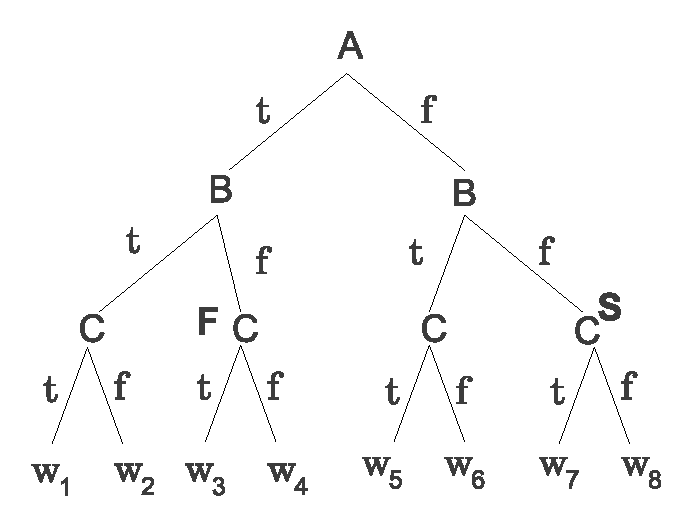
\includegraphics[width=0.5\textwidth]{searchtree}
	\caption{A search tree for the CNF $\Delta =\{\{\neg A,B\},\{\neg B,C\}\}$.}
	\label{fig:searchtree}
\end{figure}

The Davis–Putnam–Logemann–Lovel (DPLL) algorithm is the base of all modern SAT solvers. Many refinements have made to this algorithm over the last decade, which have been significant enough to change the behaviour of the algorithm, but it is still important to know it for understanding modern solvers.


\subsection{PaMiraXT}

PaMiraXT \cite{SLB09} is one of the first attempts to use a shared clause database in a parallel SAT solver.


%%%%%%%%%%%%%%%%%%%%%%%%%%%%%%%%%%%%%%%%%%%%%%%%%%%%%%%%%%%%%%%%%%%%%%%%%%%%%%%%
% Step 12: Here's the main part of your research project. We can't tell
% you what to write here... that's your job.
% 
%%%%%%%%%%%%%%%%%%%%%%%%%%%%%%%%%%%%%%%%%%%%%%%%%%%%%%%%%%%%%%%%%%%%%%%%%%%%%%%%
\chapter{Important stuff...}\label{chap:contributions}

%%%%%%%%%%%%%%%%%%%%%%%%%%%%%%%%%%%%%%%%%%%%%%%%%%%%%%%%%%%%%%%%%%%%%%%%%%%%%%%%
% Step 13: Add a conclusions chapter
%
% 
%%%%%%%%%%%%%%%%%%%%%%%%%%%%%%%%%%%%%%%%%%%%%%%%%%%%%%%%%%%%%%%%%%%%%%%%%%%%%%%%
\chapter{Conclusions}\label{chap:conclusion}

%%%%%%%%%%%%%%%%%%%%%%%%%%%%%%%%%%%%%%%%%%%%%%%%%%%%%%%%%%%%%%%%%%%%%%%%%%%%%%%%
% Step 14: Work out the bibliography
%
% 
%%%%%%%%%%%%%%%%%%%%%%%%%%%%%%%%%%%%%%%%%%%%%%%%%%%%%%%%%%%%%%%%%%%%%%%%%%%%%%%%
% Tips: 
%
% For named.bst, if I add a~\cite*{} it will add all the references I
% have in the bibliography file (whether they are referenced in the
% document or not)
%%%%%%%%%%%%%%%%%%%%%%%%%%%%%%%%%%%%%%%%%%%%%%%%%%%%%%%%%%%%%%%%%%%%%%%%%%%%%%%%
\bibliographystyle{plain}
\bibliography{biblio}

\end{document}
